\documentclass[twocolumn,10pt]{article}
\title{Area and circumference of circles}
\setlength{\columnsep}{20pt} 
\usepackage{amsmath,hyperref,cancel,graphicx}
 \def\shrinkfactor{0.55}
 \usepackage[margin=1.5cm]{geometry}
\usepackage[usenames,dvipsnames]{color}
 
 \newcommand{\blue}[1]{{\color{Blue}#1}} 
 \newcommand{\purple}[1]{{\color{Purple}#1}} 
 \newcommand{\red}[1]{{\color{Red}#1}} 
 \newcommand{\green}[1]{{\color{Green}#1}} 
 \newcommand{\gray}[1]{{\color{Gray}#1}} 
  \newcommand{\pink}[1]{{\color{Magenta}#1}}   


\begin{document}
\maketitle



\section{\href{https://www.khanacademy.org/devadmin/content/items/x067a2ea8fceec945}{x067a2ea8fceec945}}

\noindent
A python curls up to form the shape of a circle and bites the tip of its own tail. The python is $2.6 \text{ m}$ long.  

**What is the radius of the circle it forms?**  
(expression you answer in $\text{cm}$)

\paragraph{Ans} $r=$ [[? input-number 1]]  $\text{cm}$  41.4

\paragraph{Hint 1}This problem calls for the circumference formula  $\blue{C}=2\pi \red{r}$. 

\paragraph{Hint 2}When the python curls to form the shape of a circle, the circumference of this circle is equal to the length of the python $\blue{C}=\blue{2.6}\text{ m}$.

\paragraph{Hint 3}We know the formula for the circumference of a circle is $\blue{C}=2\pi \red{r}$, where $\pi = 3.14$. 

If we want to find the radius of the circle formed by the python we must solve for $\red{r}$ in the following equation 

\begin{align*}
  \qquad  2\pi \red{r} 	&= \blue{2.6}\text{ m} \\[1mm]
   \red{r}    &= \dfrac{ \blue{2.6} } { 2 \pi }\text{ m}  \\[1mm]
   \red{r}     	&= \red{0.414}\text{ m}
\end{align*}

\paragraph{Hint 4}The radius of the circle formed by the python is $\red{0.414}\text{ m}$, which is the same as $41.4 \text{ cm}$.



\medskip
\noindent
\textbf{Tags:} {\footnotesize CC.7.G.B.4, SB.7.1.F.2.SR, Area and circumference of a circle.Circle circumference}\\
\textbf{Version:} c5865da1.. 2013-09-25
\smallskip\hrule





\section{\href{https://www.khanacademy.org/devadmin/content/items/x1cfcca1f7e21f454}{x1cfcca1f7e21f454}}

\noindent
A wet bicycle tire leaves a trace of water on the floor. The tire has a radius of $14\text{ in}$ and the bicycle wheel makes $3$ full rotations before stopping. 

**How long is the trace of water left on the floor?**

\paragraph{Ans} [[? input-number 1]]  $\text{in}$  263.89378290154264

\paragraph{Hint 1}The length of the trace of water depends on the circumference of the tire. Each time the wheel rolls forward through one rotation, the tire leaves a mark with length equal to the circumference of the tire.

\paragraph{Hint 2}The circumference of a tire with radius $\red{r}=\red{14}\text{ in}$ is  

$\qquad \blue{C}=2\pi \red{r}=2\pi (\red{14}\text{ in})= \blue{28\pi}\text{ in}$. 

\paragraph{Hint 3}Since the bike wheel makes $\pink{3}$ full turns before stopping, the total length of the water trace is $\pink{3}$ times the circumference of the tire:  

$\qquad \text{length of water trace } = \pink{3}\times \blue{28\pi}\text{ in} = 84\pi  \text{ in}$.



\medskip
\noindent
\textbf{Tags:} {\footnotesize CC.7.G.B.4, SB.7.1.F.2.SR, Area and circumference of a circle.Circle circumference}\\
\textbf{Version:} 33f6d3d7.. 2013-09-25
\smallskip\hrule





\section{\href{https://www.khanacademy.org/devadmin/content/items/x1f4b934dfe143abf}{x1f4b934dfe143abf}}

\noindent
A circle with diameter $d=4$ is cut into thin slices. The slices are then rearranged so that half of the slices point downward and half point upward so they form a shape that resembles a parallelogram. Since the circle and the parallelogram are made up of the same slices, the area of the two figures is the same.


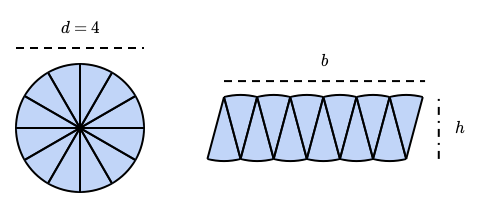
\includegraphics[scale=\shrinkfactor]{figures/de97faccd848f9b4daf365405194c42ffb713d14.png}

The radius of the circle is $r=$ [[? input-number 1]].  
Since the slices come from the circle, the height of the bumpy parallelogram is $h=$ [[? input-number 2]].  
The circumference of the circle is given by the formula $C=2\pi r$. Half the edges of the slices form the base of the parallelogram so the length of the base is equal to half the circumference $b=$ [[? input-number 3]].   
Using the formula for the area of a parallelogram, we find the area of the circle is equal to $A=b\times h=$ [[? input-number 4]].


\paragraph{Ans} Complete the sentences. 

\paragraph{Hint 1}In this exercise we will use the formula for the circumference of a circle $\blue{C}=2\pi \red{r}$ in order to derive the formula for the area of a circle $\purple{A}=\pi \red{r}^2$.

\paragraph{Hint 2}The circle has diameter $\green{d}=\green{4}$ so its radius is $\red{r}=\frac{\green{d}}{2}=\red{2}$. 

\paragraph{Hint 3}The height of the parallelogram is equal to the length of the slices. Since the slices come from the circle with radius $\red{r}=\red{2}$, the height of the parallelogram is $h=2$.

\paragraph{Hint 4}The circumference of a circle with radius $\red{r}=\red{2}$ is $\blue{C}=2\pi \red{r}=2\pi \red{2}=\blue{4\pi}$. This corresponds to the length of the edge of the circle. 

When we rearrange the slices in the parallelogram shape, the length of the base of the parallelogram is equal to half of the circumference of the circle:

$\qquad b = \dfrac{\blue{C}}{2} = \dfrac{ \blue{4 \pi}  }{2} = 2\pi$.


\paragraph{Hint 5}The area of the circle is the same as the area of the parallelogram. We can therefore find the area of the circle using the formula for the area of a parallelogram:

$\qquad A=b\times h=2\pi \times 2= 4\pi$.



\medskip
\noindent
\textbf{Tags:} {\footnotesize CC.7.G.B.4, SB.7.1.F.2.SR, Area and circumference of a circle.derive A formula from C formula}\\
\textbf{Version:} b976de6f.. 2013-09-30
\smallskip\hrule





\section{\href{https://www.khanacademy.org/devadmin/content/items/x207f8a7e9a127fad}{x207f8a7e9a127fad}}

\noindent
An engineer is planning a new water pipe installation.
The pipe has a diameter of $d=20\text{ cm}$.

**What is the area of the cross section of this pipe?**

\paragraph{Ans} $A =$ [[? input-number 1]] $\text{cm}^2$        314.1592653589793

\paragraph{Hint 1}This problem calls for the formula for the area of a circle $\purple{A} = \pi \red{r}^2$.


\paragraph{Hint 2}The diameter of the pipe is $\green{d}=\green{20}\text{ cm}$. Since the diameter of a circle is double the length of the radius, the radius of the pipe is $\red{r}=\frac{\green{d}}{2} = \red{10}\text{ cm}$.

\paragraph{Hint 3}We can now use the formula for the area of a circle $\purple{A} = \pi \red{r}^2$ to calculate the area of the pipe. The area of a pipe with radius $\red{r}=\red{10}\text{ cm}$ is

\begin{align*}
  \qquad \purple{A}  	&= \pi \red{r}^2 				\\
  		&= \pi (\red{10})^2			\\
  		&= \pi (100)		\\
  		&= 100 \pi \text{ cm}^2
\end{align*}

\paragraph{Hint 4}The area of the cross section of this pipe is $100\pi  \text{ cm}^2$. 



\medskip
\noindent
\textbf{Tags:} {\footnotesize CC.7.G.B.4, SB.7.1.F.2.SR, Area and circumference of a circle.circle area}\\
\textbf{Version:} 975543c7.. 2013-09-29
\smallskip\hrule





\section{\href{https://www.khanacademy.org/devadmin/content/items/x3879b8b46e93651e}{x3879b8b46e93651e}}

\noindent
A baker uses a coffee mug with diameter $d=8\text{ cm}$  to cut out circular cookies from a big sheet of cookie dough.  

**What is the area of each cookie?**

\paragraph{Ans} $A=$ [[? input-number 1]] $\text{cm}^2$  50.26548245743669

\paragraph{Hint 1}This problem calls for the formula for the area of a circle $\purple{A}=\pi \red{r}^2$. 

\paragraph{Hint 2}The cup has a circular shape and its diameter is $\green{d}=\green{8}\text{ cm}$.

The radius of the cup is 

$\qquad \red{r} = \dfrac{\green{d}}{2}= \dfrac{\green{8}\text{ cm}}{2}=\red{4}\text{ cm}$.

To find the area, we can substitute the value $\red{r} = \red{4}\text{ cm}$ into the formula for the area of a circle.

\paragraph{Hint 3}We now use the formula  $\purple{A}=\pi \red{r}^2$ to find the area of each cookie:

\begin{align*}
 \qquad \purple{A} 	& =\pi \red{r}^2 	\\
  	& = \pi (\red{4}\text{ cm})^2		\\
  	& = \pi (\red{4} \times \red{4}) \text{ cm}^2		\\
  	&= 16 \pi  \text{ cm}^2		
\end{align*}

The area of each cookie is  $16 \pi \text{ cm}^2$.



\medskip
\noindent
\textbf{Tags:} {\footnotesize CC.7.G.B.4, SB.7.1.F.2.SR, Area and circumference of a circle.circle area}\\
\textbf{Version:} c4e60616.. 2013-09-25
\smallskip\hrule





\section{\href{https://www.khanacademy.org/devadmin/content/items/x4d9ac4ed5246f99b}{x4d9ac4ed5246f99b}}

\noindent
Your local pizza place offers the following two deals each priced at $\$25$.  
Option 1: One extra-large pizza with diameter $20\text{ in}$.  
Option 2: Two medium pizzas with diameter $15\text{ in}$ each.

**Which of the options offers a lower price per square inch of pizza?**


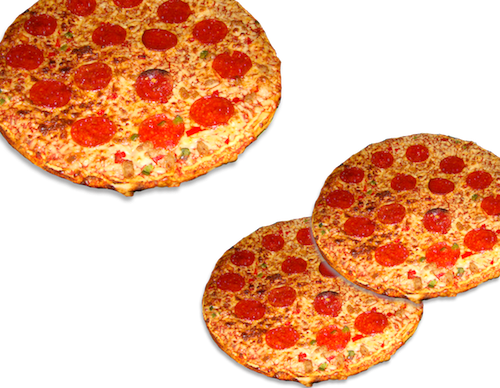
\includegraphics[scale=\shrinkfactor]{figures/5ac1d9f5c91daf1f9f7c2bcb006c279c70abc72a.png}

\paragraph{Ans} Option 1 costs [[? input-number 1]] cents per square inch.  
Option 2 costs [[? input-number 2]] cents per square inch, 
so [[? dropdown 1]] has a lower price per square inch.  8

\paragraph{Hint 1}Let's use the area formula $\purple{A}=\pi \red{r}^2$ to find the price per square inch for the two deals. We'll use the approximation $\pi=3.14$ in this problem.

Since the price of both options is the same, we just have to compare the total area of pizza in each option.

\paragraph{Hint 2}For Option 1, the total area of pizza is equal to the area of the extra-large pizza 

\begin{align*}
\qquad A_1 
  &= A_{\text{extra-large}}  \\
  &= \pi \red{r}^2  \\
  & = \pi (\red{10})^2  \\
  &= \pi 100  \\
  &= 314\text{ in}^2
\end{align*}

\paragraph{Hint 3}For Option 2, the total area of pizza is the sum of the areas of the two medium pizzas

\begin{align*}
\qquad A_2 
 &= \blue{2}A_{\text{medium}} \\
  &= \blue{2}\left[\pi \red{r}^2 \right] \\
 &= \blue{2}\left[\pi (\red{7.5})^2\right]  \\
 &= \blue{2}\left[\pi  56.25 \right]  \\
 &= 353.25\text{ in}^2
\end{align*}


\paragraph{Hint 4}What is the price per square inch of pizza for the two options? 

The price per square inch for Option 1 is  

$\qquad \dfrac{\$25}{A_1} = \dfrac{\$25}{314\text{ in}^2} =0.0796\:\dfrac{\$\ \ }{\text{in}^2}$

The price per square inch for Option 2 is  

$\qquad \dfrac{\$25}{A_2} = \dfrac{\$25}{353.25\text{ in}^2} =0.0707\:\dfrac{\$\ \ }{\text{in}^2}$

\paragraph{Hint 5}Rounding the prices to the nearest cent, Option 1 costs  $\mathbf{8}$ cents per square inch, while Option 2 is $\mathbf{7}$ cents per square inch. **Option 2** has a  lower price per square inch. 



\medskip
\noindent
\textbf{Tags:} {\footnotesize CC.7.G.B.4, SB.7.1.F.2.SR, Area and circumference of a circle.circle area}\\
\textbf{Version:} fbd5ca17.. 2013-09-25
\smallskip\hrule





\section{\href{https://www.khanacademy.org/devadmin/content/items/x560d92c3a06b1431}{x560d92c3a06b1431}}

\noindent
What is the ratio between a circle's circumference $C$ and its diameter $d$?


\paragraph{Ans} $\dfrac{C}{d} = $ [[? input-number 1]]   3.141592653589793

\paragraph{Hint 1}This question tests your knowledge of the formula for the circumference of a circle. 

\paragraph{Hint 2}The circumference of a circle with diameter  $\green{d} $ is $\blue{C}=\pi \green{d}$. 

The ratio of the circle's circumference to the circle's diameter is therefore  

$\qquad \dfrac{\blue{C}}{\green{d}}=\pi$. 

\paragraph{Hint 3}In fact, this is how the number $\pi$ is defined.
The number $\pi = 3.14159265\ldots$ is defined as the ratio between the circumference and the diameter of *any* circle**.**
 



\medskip
\noindent
\textbf{Tags:} {\footnotesize CC.7.G.B.4, SB.7.1.F.2.SR, Area and circumference of a circle.Circle circumference}\\
\textbf{Version:} a0af47db.. 2013-09-30
\smallskip\hrule





\section{\href{https://www.khanacademy.org/devadmin/content/items/x790eb845d377100f}{x790eb845d377100f}}

\noindent
**Find the area of the shaded region.**


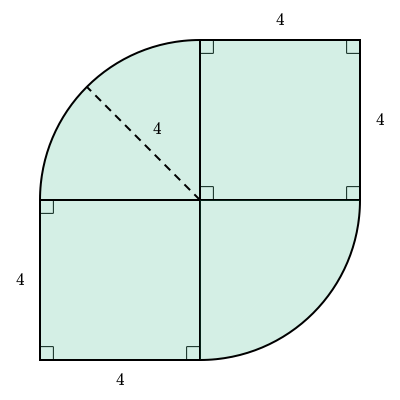
\includegraphics[scale=\shrinkfactor]{figures/eb8635a8059b2c69ad19bf8d44f5a7a7885cf622.png}


\paragraph{Ans} $A =$ 
[[? expression 1]]  32 + 8*pi

\paragraph{Hint 1}The region is a combination of two squares and two quarters of a circle. 
The two squares have side length $\pink{4}$.
The circular sections have radius $\purple{r}=\purple{4}$.

To find the area of the region we can find the area of each of its parts and then add the areas. 

\paragraph{Hint 2}There are two squares in the figure and their total area is 

$\qquad \red{A}=2\times (\pink{4}\times \pink{4}) = \red{32}$.

\paragraph{Hint 3}The circular regions are quarters of a circle. The area of a whole circle is $\pi\purple{r}^2$ so the area of a quarter circle is $\frac{1}{4}$ of $\pi \purple{r}^2$.

The radius of the circular regions is $\red{r}=\red{4}$ and there are $2$ circular parts so their combined area is 

 $\qquad \blue{A} = 2 \times (\frac{1}{4}\pi \purple{r}^2) = \frac{1}{2} \pi \purple{4}^2 = \blue{8\pi}$.


\paragraph{Hint 4}
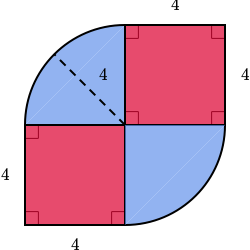
\includegraphics[scale=\shrinkfactor]{figures/be75119c9ec750491ada6dd94f5083c448ab9aad.png} 

The total area of the region is the area of the square parts plus the area of the circular parts:

$\qquad A = \red{32} + \blue{8\pi}$.





\medskip
\noindent
\textbf{Tags:} {\footnotesize CC.7.G.B.4, Area and circumference of a circle.Composite region calculations, SB.7.1.F.2.SR}\\
\textbf{Version:} e99b0573.. 2013-09-30
\smallskip\hrule





\section{\href{https://www.khanacademy.org/devadmin/content/items/x96a8cbf4fb017d88}{x96a8cbf4fb017d88}}

\noindent
A compact-disk (CD) has a diameter of $12\text{ cm}$. The hole in the middle has a diameter of $1.5\text{ cm}$. 

**What is the area of the disk?**  


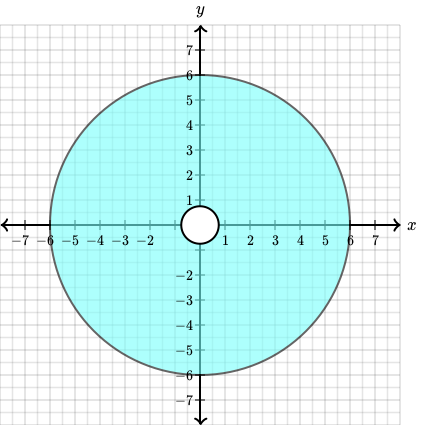
\includegraphics[scale=\shrinkfactor]{figures/4a4b7babd816aab550a5ae1cb6753bb6e7eacad6.png}

\paragraph{Ans} $A =$ [[? input-number 1]] $\text{cm}^2$  111.33018966158829

\paragraph{Hint 1}The area of a CD is equal to the total area the disk minus the area of the hole in the middle.

\paragraph{Hint 2}We need to use the formula for the area of a circle $\purple{A} = \pi \red{r}^2$ two times.

The outer radius of the disk is $\red{r} = \frac{\green{d}}{2}=\frac{\green{12}\text{ cm}}{2}=\red{6}\text{ cm}$, so the area of the disk (including the hole) is   

\begin{align*}
  \qquad \purple{A}_{\text{outer}}  	&= \pi \red{r}^2 			\\
  		&= \pi (\red{6}\text{ cm})^2			\\
  		&= \pi (\red{6} \times \red{6}) \text{ cm}^2			\\
  		&= 36 \pi  \text{ cm}^2		
\end{align*}

\paragraph{Hint 3}The radius of the hole in the middle is $\red{r} = \frac{\green{d}}{2}= \frac{\green{1.5}\text{ cm}}{2}=\red{0.75}\text{ cm}$, so the area of the hole is
 
\begin{align*}
  \qquad \purple{A}_{\text{hole}}  	&= \pi \red{r}^2 				\\
  		&= \pi (\red{0.75}\text{ cm})^2			\\
  		&= \pi (\red{0.75} \times \red{0.75}) \text{ cm}^2			\\
  		&= \pi \left(\red{\frac{3}{4}} \times \red{\frac{3}{4}}\right) \text{ cm}^2			\\
  		&= \frac{9\pi}{16} \text{ cm}^2		
\end{align*}

\paragraph{Hint 4}The area of the CD is  

\begin{align*}
\quad \purple{A}_{\text{CD}} 
  &= \purple{A}_{\text{outer}} - \purple{A}_{\text{hole}} \\[2mm] 
  &= 36\pi -  \frac{9\pi}{16}  \\[1.2mm]
  &= \left(36 -  \frac{9}{16}\right)\pi  \\[1.2mm]
  &= \left(\frac{36\times\blue{16}}{\blue{16}} -  \frac{9}{16}\right)\pi  \\[1.2mm]
  &= \left(\frac{576}{16} -  \frac{9}{16}\right)\pi  \\[1.2mm]
  &= \frac{567\pi}{16} \text{ cm}^2.
\end{align*}

\paragraph{Hint 5}We obtain the final answer $A_{\text{CD}}=\frac{567\pi}{16}\text{ cm}^2$, which is approximately equal to $111.3\text{ cm}^2$.



\medskip
\noindent
\textbf{Tags:} {\footnotesize CC.7.G.B.4, SB.7.1.F.2.SR, Area and circumference of a circle.circle area}\\
\textbf{Version:} 5889ae7c.. 2013-09-25
\smallskip\hrule





\section{\href{https://www.khanacademy.org/devadmin/content/items/x9a3db47ccf936b4a}{x9a3db47ccf936b4a}}

\noindent
A pizza of radius $r$, diameter $d=2r$, and circumference $2\pi r$ is cut into thin slices. The slices are then placed so they form a shape that resembles a parallelogram. The area of the parallelogram is the same as the area of the pizza.


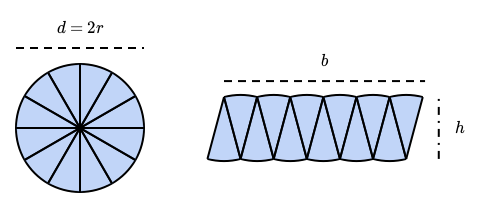
\includegraphics[scale=\shrinkfactor]{figures/3f15087165055ef8a63a60583da95a017c9259b9.png}

In the new arrangement of the slices, the crust of the pizza forms the bottom and top edges of the parallelogram. The length of the base of the parallelogram is equal to half of the circumference of the pizza $b=$ [[? dropdown 1]].  
The height $h$ of the parallelogram is equal to the lengths of the pizza slices $h=$ [[? dropdown 2]].  
Using the formula for the area of a parallelogram $A=b\times h$, we find the area of the pizza is equal to $A=$ [[? dropdown 3]].

\paragraph{Ans} Complete the sentences. 

\paragraph{Hint 1}In this exercise we will use the formula for the circumference of a circle $\blue{C}=2\pi \red{r}$ in order to derive the formula for the area of a circle $\purple{A}=\pi \red{r}^2$.

\paragraph{Hint 2}We know the circumference of a circle of radius $\red{r}$ is $\blue{C}=2\pi \red{r}$. The total length of the crust of a pizza with radius $\red{r}$ is $2\pi \red{r}$.

When we rearrange the slices in the parallelogram shape, the length of the base of the parallelogram is equal to half of the circumference of the pizza:

$\qquad b = \dfrac{\blue{C}}{2} = \dfrac{ 2 \pi \red{r} }{2} = \pi \red{r}$.

\paragraph{Hint 3}The height of the parallelogram is equal to the length of the pizza slices. Since the slices come from a pizza with radius $\red{r}$, the length of each pizza slice is $\red{r}$. Thus, the height of the parallelogram is $h=\red{r}$.

\paragraph{Hint 4}The area of the pizza is the same as the area of the parallelogram. We can therefore find the area of the pizza by using the formula for the area of a parallelogram $A=b\times h$. 

The area of a circle of radius $\red{r}$  is $A=\pi\red{r}\times \red{r}=\pi \red{r}^2$.

\paragraph{Hint 5}The length of the base of the parallelogram is $b=\pi\red{r}$. The height $h$ of the parallelogram is  $h= \red{r}$. The area of the pizza is equal to $A=\pi \red{r}^2$.



\medskip
\noindent
\textbf{Tags:} {\footnotesize CC.7.G.B.4, SB.7.1.F.2.SR, Area and circumference of a circle.derive A formula from C formula}\\
\textbf{Version:} b88e4fdd.. 2013-09-24
\smallskip\hrule





\section{\href{https://www.khanacademy.org/devadmin/content/items/xa9879653bc4a66ea}{xa9879653bc4a66ea}}

\noindent
If the radius of a circle is multiplied by a factor of 2, by what factor will the area of the circle increase?

\paragraph{Ans} The area is [[? input-number 1]] times bigger  4

\paragraph{Hint 1}Let's look at the formula for the area of a circle $A=\pi r^2$. 
How will the area change if we replace $r$ with $2r$?

\paragraph{Hint 2}The area of a circle with radius $2r$ is 

\begin{align*}
\qquad \pi (2r)^2 
  & =\pi(2r)(2r) \\
  &=\pi(2 \times 2 \times r \times r)  \\
   &= \pi \times 4 \times r^2 \\
   &= 4\pi r^2
\end{align*} 

which is 4 times bigger than the area of a circle of radius $r$. 


\paragraph{Hint 3}When the radius of a circle doubles, the area increases $4$ times because the radius $r$ is squared in the formula $A=\pi r^2$.




\medskip
\noindent
\textbf{Tags:} {\footnotesize CC.7.G.B.4, SB.7.1.F.2.SR, Area and circumference of a circle.circle area}\\
\textbf{Version:} e5d9081c.. 2013-09-16
\smallskip\hrule





\section{\href{https://www.khanacademy.org/devadmin/content/items/xade69580de9f3c4e}{xade69580de9f3c4e}}

\noindent
**Find the area of the shaded region.**


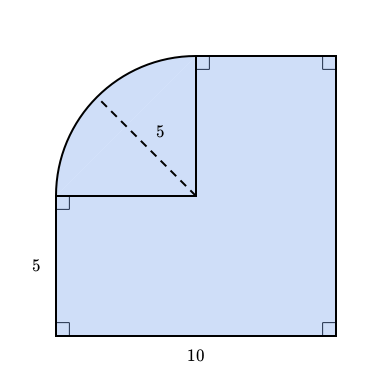
\includegraphics[scale=\shrinkfactor]{figures/b0216381822fdf828c9b1c0c60a3da3a18cdb9da.png}


\paragraph{Ans} $A =$ 
[[? expression 1]]  75 + 25*pi/4

\paragraph{Hint 1}The region in the figure is a combination of an $L$-shaped polygon with right angles and a quarter circle.  The quarter circle has radius $r=5$.

To find the total area of the region we can split it up into parts and then add the areas of the parts.

\paragraph{Hint 2}The curved part is a quarter circle. The area of a whole circle is $\pi r^2$. The area of quarter circle is $\frac{1}{4}$ of $\pi r^2$.

The radius of the circular regions is $r=5$ so the area of a quarter circle is

\begin{align*} 
\qquad \green{A} &= \frac{1}{4}\pi r^2 \\[1mm]
&= \frac{1}{4} \pi 5^2 \\[2mm]
&= \green{\dfrac{25\pi}{4}}
\end{align*}


\paragraph{Hint 3}We can decompose the rest of the region into a rectangle and a square. 

First calculate the are area of the rectangular region:
The area of this rectangular region is 

$\qquad \red{A}=5\times 10 = \red{50}$.

Next we calculate the area of the square region.
The square has side length $5$ so the its area is  

$\qquad \purple{A}=5\times 5 = \purple{25}$.


\paragraph{Hint 4}The total area of the shaded region is the sum of the area of the $\green{\text{quarter circle}}$, the area of the $\red{\text{rectangular region}}$, and area of the $\purple{\text{square region}}$:

\begin{align*}
\qquad A &= \green{\dfrac{25\pi}{4}} + \red{50} + \purple{25}\\ &=  \dfrac{25\pi}{4}+ 75.
\end{align*}


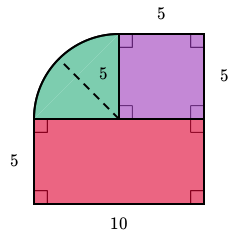
\includegraphics[scale=\shrinkfactor]{figures/5505e58c694464279f963187f09c2f77d54a9a63.png} 

The total area of the shaded region is $A=\dfrac{25\pi}{4}+ 75$.



\medskip
\noindent
\textbf{Tags:} {\footnotesize CC.7.G.B.4, Area and circumference of a circle.Composite region calculations, SB.7.1.F.2.SR}\\
\textbf{Version:} 77dd1e24.. 2013-09-29
\smallskip\hrule





\section{\href{https://www.khanacademy.org/devadmin/content/items/xb4dd0f0616538444}{xb4dd0f0616538444}}

\noindent
The circumference of a circle $C$ is proportional to the circle's diameter $d$.

**What is the constant of proportionality?**

\paragraph{Ans} $C= $ [[? input-number 1]]$d$   3.141592653589793

\paragraph{Hint 1}This question tests your knowledge of the formula for the circumference of a circle. 

\paragraph{Hint 2}The circumference of a circle with diameter  $\green{d} $ is $\blue{C}=\pi \green{d}$.  The bigger the diameter, the bigger the circumference. 

We can find the constant of proportionality by dividing the circumference by the diameter 

$\qquad \dfrac{\blue{C}}{\green{d}}=\pi$. 



\paragraph{Hint 3}This is how the number $\pi$ is defined.
The number $\pi = 3.14159265\ldots$ is defined as the constant of proportionality which relates the circle's diameter to its circumference**.**
 



\medskip
\noindent
\textbf{Tags:} {\footnotesize CC.7.G.B.4, SB.7.1.F.2.SR, Area and circumference of a circle.Circle circumference}\\
\textbf{Version:} a1c044c5.. 2013-09-30
\smallskip\hrule





\section{\href{https://www.khanacademy.org/devadmin/content/items/xb9d0da8f1cff505a}{xb9d0da8f1cff505a}}

\noindent
Lucy wants to calculate the area of a $14\text{ in}$ pizza, but she forgot the formula for the area of a circle. After cutting the pizza into slices, she decides to rearrange the slices so that half the slices point downward and half point upward as shown in the figure. The pizza now looks like a parallelogram and the area of the parallelogram is the same as the area of the circle. Lucy uses a ruler to measure the length of the base of this parallelogram and its height.


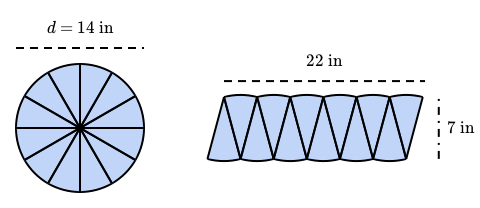
\includegraphics[scale=\shrinkfactor]{figures/d9c172d7729db26550c8739d81ac4ffe0918907f.png}

The length of the base of the parallelogram is $b=$ [[? input-number 1]] $\text{in}$ 
and its height is $h=$ [[? input-number 2]] $\text{in}$. The area of a parallelogram is equal to the length of its base times its heights $A=b\times h$. The area of the circle is therefore $A=$ [[? input-number 3]] $\text{in}^2$. 

\paragraph{Ans} Complete the sentences. 

\paragraph{Hint 1}In this exercise we will use the formula for the area of a parallelogram $A=b\times h$ in order to find the area of a circle.

\paragraph{Hint 2}The area of a parallelogram is equal to the length of its base times its heights $A=b\times h$.

The length of the base of the parallelogram is $b=22\text{ in}$ and its height is $h=7\text{ in}$, therefore its area is 

$\qquad A= b \times h = 22 \times 7 = 154\text{ in}^2$ 

\paragraph{Hint 3}**Since the circle and the parallelogram are made up of the same slices, the area of the circle is approximately equal to $154\text{ in}^2$.**

Note we could obtain the same number using the formula for the area of a circle $A=\pi r^2=\pi (7)^2 = 49\pi \text{ in}^2$. Using the approximation $\pi=3.14$ we find $A=49\pi=153.86\text{ in}^2$, which is pretty close to what Lucy obtained using her method.



\medskip
\noindent
\textbf{Tags:} {\footnotesize CC.7.G.B.4, SB.7.1.F.2.SR, Area and circumference of a circle.derive A formula from C formula}\\
\textbf{Version:} 15eb98db.. 2013-09-25
\smallskip\hrule





\section{\href{https://www.khanacademy.org/devadmin/content/items/xc36d0fcab2738fb5}{xc36d0fcab2738fb5}}

\noindent
A building engineer is analyzing a concrete column which has a circular cross section. 
Using a measuring tape, he finds the circumference of the column is $C =18\text{ m}$. 

**What is the area of the cross section of the column?**

\paragraph{Ans} $A =$ [[? input-number 1]]  $\text{m}^2$  25.79

\paragraph{Hint 1}The cross section of the concrete column is a circle. The engineer knows the circumference of the circle and wants to find the area. 

We must combine the formulas $\blue{C}=2\pi \red{r}$ and $\purple{A}=\pi \red{r}^2$ to solve this problem.

\paragraph{Hint 2}The circumference of a circle with radius $\red{r}$ is $\blue{C}=2\pi \red{r}$. 
Since we know $\blue{C}=18\text{ m}$, we can find $\red{r}$ by solving the following equation:

\begin{align*}
   \qquad 2\pi \red{r} 	&= \blue{18} \text{ m}	\\[1mm]
   \red{r}     	&= \dfrac{ \blue{18} } { 2 \pi } 	\\[1mm]
   \red{r}     	&= \red{2.866}\text{ m}
\end{align*}

\paragraph{Hint 3}Now that we know the radius of the column is $\red{r}=\red{2.866}\text{ m}$, we can find the area of the cross section: 

\begin{align*}
 \qquad \purple{A} 	& =\pi \red{r}^2 					\\
  			& = \pi (\red{2.866}\text{ m})^2			\\
  			& = 3.14 (\red{2.866}\text{ m})^2			\\  
			& = 25.79 \text{ m}^2
\end{align*}



\medskip
\noindent
\textbf{Tags:} {\footnotesize CC.7.G.B.4, SB.7.1.F.2.SR, Area and circumference of a circle.Circle circumference}\\
\textbf{Version:} da249326.. 2013-09-16
\smallskip\hrule





\section{\href{https://www.khanacademy.org/devadmin/content/items/xe448997a086976be}{xe448997a086976be}}

\noindent
An engineer is tasked to install a pipe which supplies the water to a building.
The new pipe must have a cross-sectional area of $A=100\pi \text{ cm}^2$.

**What diameter of pipe should the engineer choose?**

\paragraph{Ans} $d=$  [[? input-number 1]]  $\text{cm}$  20

\paragraph{Hint 1}This problem calls for the area formula for a circle $\purple{A} = \pi \red{r}^2$. 
We know the cross-sectional area of the pipe is  $\purple{A}=\purple{100\pi }\text{ cm}^2$
and we want to find the diameter of the pipe.

\paragraph{Hint 2}We can find the radius of the pipe if we solve for $\red{r}$ in the following equation  

\begin{align*}
 \qquad  \pi \red{r}^2  &= \purple{100\pi} \text{ cm}^2			\\
  \pi \red{r}^2 	&= 10^2\pi 			\\
   \cancel{\pi} \red{r}^2 	&= 10^2\cancel{\pi} 			\\
   \red{r}^2     			&= 10^2 				\\
   \red{r}     			&= \red{10}\text{ cm}
\end{align*}

Note the reasoning we used in the last step: $\red{r}^2=10^2$, therefore $\red{r}=\red{10}$. 
Since the area is measured in $\text{cm}^2$ the radius is measured in $\text{cm}$.

\paragraph{Hint 3}Since the diameter of the pipe is double the length of the radius, the diameter of the pipe must be $\green{d} = 2\red{r}=2\cdot\red{10} = \green{20}\text{ cm}$.



\medskip
\noindent
\textbf{Tags:} {\footnotesize CC.7.G.B.4, SB.7.1.F.2.SR, Area and circumference of a circle.circle area}\\
\textbf{Version:} 4f7d4cb3.. 2013-09-29
\smallskip\hrule





\section{\href{https://www.khanacademy.org/devadmin/content/items/xe76e25d5bcae424a}{xe76e25d5bcae424a}}

\noindent
The illustration below shows an office table viewed from above.  

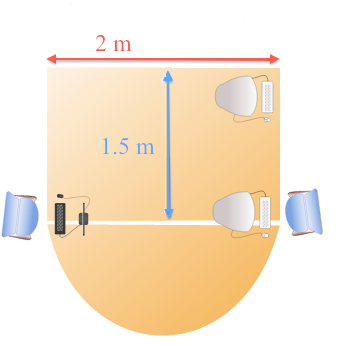
\includegraphics[scale=\shrinkfactor]{figures/2e7c87313a5fdbe0bacdee8a3f8f46418add2f40.png}

**What is the total area of the table?**  
Give your answer as a decimal and use the approximation $\pi=3.14$.

\paragraph{Ans} $A=$ [[? input-number 1]] $\text{m}^2$  4.57

\paragraph{Hint 1}The total area of the table is equal to the area of the rectangular part of the table plus the area of the circular part.

\paragraph{Hint 2}The area of a rectangle is equal to the width of the  rectangles times its height $A=\red{w}\times \blue{h}$. 

Therefore the rectangular part of the table has area 

$\qquad A = \red{2}\text{ m} \times \blue{1.5}\text{ m} = 3\text{ m}^2$

\paragraph{Hint 3}The circular part of the table has the shape of a half-circle with diameter $\red{d}=\red{2}\text{ m}$. If the diameter of a circle is $\red{d}=\red{2}\text{ m}$ then its radius is $\green{r}=\green{1}\text{ m}$ and its area is $A=\pi \green{r}^2=\pi\text{ m}^2$.

The area of the circular part of the table is equal to $\purple{\text{half}}$ of the area of the full circle:

$\qquad A 
= \purple{\dfrac{1}{2}}\pi\green{r}^2
= \purple{\dfrac{1}{2}}\pi(\green{1})^2
= \dfrac{\pi}{2}\text{ m}^2 $



\paragraph{Hint 4}The total area of the table is the sum of the areas of the  rectangular and the circular parts of the table:

\begin{align*}
\qquad A_{\text{table}} 
&= 3\text{ m}^2 + \dfrac{\pi}{2} \text{ m}^2 \\
&= \left(3+\dfrac{\pi}{2}\right)\text{ m}^2
\end{align*}



\paragraph{Hint 5}Using the approximation $\pi=3.14$ we find the area of the table is 

$\qquad A_{\text{table}} = \left(3+\dfrac{3.14}{2}\right) = 4.57\text{ m}^2$




\medskip
\noindent
\textbf{Tags:} {\footnotesize CC.7.G.B.4, Area and circumference of a circle.Composite region calculations, SB.7.1.F.2.SR}\\
\textbf{Version:} 8e03e611.. 2013-09-30
\smallskip\hrule





\section{\href{https://www.khanacademy.org/devadmin/content/items/xefc631c99946d20d}{xefc631c99946d20d}}

\noindent
**Find the area of the shaded region.**


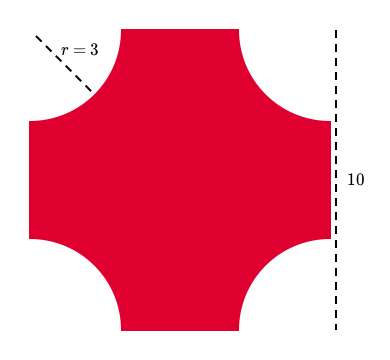
\includegraphics[scale=\shrinkfactor]{figures/ec1d9546c0b030bf9e41bb394bf1c4337b8a1c2c.png}

\paragraph{Ans} $A =$ [[? input-number 1]]  71.7256661177

\paragraph{Hint 1}The area of the shaded region looks like a square with the four corners cut out. Each of the corners is one quarter of a circle. Thus, to find the area of the shaded region we must find the area of the square and subtract the area that is missing from the four corners.

\paragraph{Hint 2}The area of the square (including the corners) is   

$\qquad \purple{A}=10\times 10 = \purple{100}$.

\paragraph{Hint 3}Each of the corners is a quarter circle with radius $\red{r}=\red{3}$, and there are four corners so the total area that is missing is equal to the area of one whole circle with radius $\red{r}=\red{3}$.
The area of a circle of radius $\red{3}$ is 

 $\qquad \blue{A} = \pi (\red{r})^2 = \pi \red{3}^2 = \blue{9\pi}$.

\paragraph{Hint 4}Therefore, the area of the shaded region is equal to $\purple{100} - \blue{9\pi}$.



\medskip
\noindent
\textbf{Tags:} {\footnotesize CC.7.G.B.4, Area and circumference of a circle.Composite region calculations, SB.7.1.F.2.SR}\\
\textbf{Version:} 78a89b3e.. 2013-09-30
\smallskip\hrule



%%  Create a directory called 'figures' in latex dir and run the following command 
%  wget \
%    https://ka-perseus-graphie.s3.amazonaws.com/de97faccd848f9b4daf365405194c42ffb713d14.png \
%    https://ka-perseus-images.s3.amazonaws.com/5ac1d9f5c91daf1f9f7c2bcb006c279c70abc72a.png \
%    https://ka-perseus-graphie.s3.amazonaws.com/eb8635a8059b2c69ad19bf8d44f5a7a7885cf622.png \
%    https://ka-perseus-graphie.s3.amazonaws.com/be75119c9ec750491ada6dd94f5083c448ab9aad.png \
%    https://ka-perseus-graphie.s3.amazonaws.com/4a4b7babd816aab550a5ae1cb6753bb6e7eacad6.png \
%    https://ka-perseus-graphie.s3.amazonaws.com/3f15087165055ef8a63a60583da95a017c9259b9.png \
%    https://ka-perseus-graphie.s3.amazonaws.com/b0216381822fdf828c9b1c0c60a3da3a18cdb9da.png \
%    https://ka-perseus-graphie.s3.amazonaws.com/5505e58c694464279f963187f09c2f77d54a9a63.png \
%    https://ka-perseus-graphie.s3.amazonaws.com/d9c172d7729db26550c8739d81ac4ffe0918907f.png \
%    https://ka-perseus-images.s3.amazonaws.com/2e7c87313a5fdbe0bacdee8a3f8f46418add2f40.png \
%    https://ka-perseus-graphie.s3.amazonaws.com/ec1d9546c0b030bf9e41bb394bf1c4337b8a1c2c.png \


\end{document}